\section{FSW Execution Backup and Restore}\label{sec:das-exec-restore}
In \autoref{sec:bbpsim-charact}, the most important characteristics of the BBPSim environment were discussed. In particular, it was seen that the flight software was a multithreaded application running inside the \gls{BBPSim} environment. Because simulations had to run on a Linux machine, the re-implementation of the threading API by BBPSim was built on top of the POSIX threads library (\textit{pthread}), which is extensively supported by Linux. 

Saving the execution "point" of each thread was an important part of the design of the checkpointing feature in BBPSim. At restore time, it was vital to put back the threads' execution to the point they were in the code. However, playing with threads was not trivial, since they are an entity that is mostly abstracted in C code.

In this section, some approaches that attempted to resolve the execution restore problem are first of all described, along with why they didn't work or couldn't apply in the case of BBPSim. Then, a description of the checkpointing, saving and restoring operations that were adopted in this thesis is given, together with how they justify the addition of the last two necessary conditions (2 and 3) given in \autoref{sec:conditions}. 

\subsection*{Possible Solutions}
For simplicity purposes, it is often more useful to reduce the complexity of the problem and then scale up the solution to apply it in the real world. In the case of this thesis, the single-thread restore had to first be solved before attacking the multithread aspect. 

Inside a simulation, when monitoring between steps, a flight software thread in BBPSim could hold one of three possible states:
\begin{itemize}
	\item \textbf{Fresh}. This meant the thread was created (using the Deos API function \texttt{createThread()}) at the previous step but never actually given CPU time to execute. The thread is pending on a signal (a semaphore).
	\item \textbf{Mature}. The thread has executed for at least one step. This implies that it called \texttt{waitUntilNextPeriod()} at least once.
	\item \textbf{Dead}. This meant the thread was terminated at the last step, either by itself or another running thread.
\end{itemize}

Three different strategies were attempted to solve the execution restoring problem. One can take \autoref{code:example-task} on page \pageref{code:example-task} as an example of a flight task loop.
\begin{enumerate}
	\item \textbf{Restart back mature threads from scratch}. This had obvious problems.  Cold-starting all the threads alive when restoring would mean the task preamble (everything \textit{before} the infinite loop) would get executed twice: once at the first simulation and a second time when restoring. Since embedded utilities like mutexes also got restored, the flight software would try to re-create them when restoring. This would inevitably create runtime errors.
	
	\item \textbf{"Replay" the mature threads until their first \texttt{waitUntilNextPeriod()}}. This implied that the \texttt{create*()} Deos API functions had to somehow be "skipped", such that no embedded utility was created. The thread would then be replayed until its \texttt{waitUntilNextPeriod()}.
	
	Since \gls{BBPSim} was an \gls{ELF} dynamic library, this option consisted in hooking on these API calls, and redirecting them to stub functions that did nothing. The strategy was possible by using a complex set of operations that overwrote addresses in the look-up table used to resolve dynamic library function addresses, the \texttt{.rel.plt} section.\cite{online:shoumikhin}.
	
	This would have been a good solution, if only for the fact that tasks could contain more than one \texttt{waitUntilNextPeriod()}. There was nothing prohibiting a task to call \texttt{waitUntilNextPeriod()} in its preamble, for example. There was actually many occurrences of this in the flight software, for instance when threads wait for messages from other threads before starting their own task loop.
	
	With this in mind, it was necessary to find out at \textit{which} instance of \texttt{waitUntilNextPeriod()} the thread was saved, and when exactly should the Deos API be "re-enabled". This was considered as a poor approach with too many corner cases to implement effectively.
	
	\item \textbf{Reconstruct the entire threads}. This was the candidate kept for this thesis. Choosing this solution implied that everything required to reconstruct the thread needed to be included in the checkpointing artifact, hence the last two necessary conditions of \autoref{sec:conditions}. 
	
	The process relied on two facts: 1.\pathmono{libBbpSim.so} was always loaded at the same address by the dynamic linker and 2. both saved and restored simulations were ran on the same x86-64 machine. 
\end{enumerate}

In the previous sections, it was seen that, to restore back a simulation to its previous state, one had to backup two components pertaining to flight software execution: 1. one set of CPU registers per thread and 2. one execution stack per thread. In the following sections, the strategy used to gather these components is further detailed.

\subsection*{Checkpointing the CPU Register Set}
The first step in saving a thread's execution state was to come up with a way to make the flight software code checkpoint itself. In particular, it was important to obtain a set of registers associated with that thread at the end of every simulation step.

Saving such a register set was absolutely necessary to restore the flight threads without stability issues. The registers contained very important information about what the thread was doing. In particular, this set contained the \textit{program counter}, pictured in \autoref{fig:x86-regs}, which itself held the address of the machine instruction the thread would be currently executing. The register set also contained the stack pointer, which pointed on top of the thread's execution stack.

For obvious reasons, it was vital to save this register set \textit{at the right time} in the execution. If the registers were snapshotted at the wrong moment, the program counter would not be pointing to a viable instruction, which would make the restore operation crash. This problem was highlighted by the thread scheduling approach implemented by BBPSim. In \autoref{fig:step-cmd}, it was shown that flight software threads were executed one after another at every simulation step. In practice, this mechanism was implemented with two semaphores. The thread was pending on a "go" semaphore inside BBPSim's \texttt{waitUntilNextPeriod()} reimplementation. Once the scheduler signaled the semaphore, the thread executed a task loop until it returned inside the \texttt{waitUntilNextPeriod()} function, which signaled back to the scheduler that the thread was done. This procedure is shown in \autoref{code:thr-sched-bbpsim}.

\begin{listing}[htpb]
	\centering
	\begin{minipage}{.5\textwidth}
	\begin{minted}{c}
void Task() {
	//task premable here
	
	while(true) {
		//task loop content here
		waitUntilNextPeriod();
	}
}
	\end{minted}
	\end{minipage}%
	\begin{minipage}{.5\textwidth}
	\begin{minted}{c}
//re-implementation of Deos API
void waitUntilNextPeriod() {
	//loop finished, signal returned
	sem_post(&return_sem);
	//wait for go from scheduler 
	sem_wait(&go_sem);
}
	\end{minted}
	\end{minipage}
	\caption{Thread scheduling procedure in BBPSim.}
	\label{code:thr-sched-bbpsim}
\end{listing}

If the register snapshot happened after a simulation step (using \mintinline{c}|ptrace()| like \gls{CRIU} in \autoref{sec:criu}), all the threads would be waiting inside the \mintinline{c}{sem_wait()} function, which relied on a semaphore artifact that would not be valid anymore at restore time. Therefore, another approach was needed.

The solution chosen for this problem needed the thread to checkpoint \textit{itself}, in order to gather its own set of registers from within its own domain (i.e. inside DAS code). Requirement U02 did however forbade any modification to the flight software. Consequently, the injection of checkpointing code within the flight software was taken as the main strategy. By redefining the \texttt{waitUntilNextPeriod()} symbol, it was possible to inject code that would save the registers at the right moment. This could be done by using the compiler's preprocessor to convert source code before actually compiling the code, like in \autoref{code:chkpt-inject}. By harnessing the GNU C library's types and functions for user-implemented context switching\cite{online:getcontext}, this injection would transform the flight software \ul{at compilation} to checkpoint itself at the end of every loop, before calling the real \texttt{waitUntilNextPeriod()}. 
\begin{listing}[htpb]
	\centering
	\begin{minted}{c}
#define waitUntilNextPeriod()                         \
do                                                    \
{                                                     \
	ucontext_t* chkpt = GetThreadCheckpointSaveSlot();\
	getcontext(chkpt);                                \
	waitUntilNextPeriodReal();                        \ 
} while(0)

void waitUntilNextPeriodReal() //<- redefined
{
	//semaphore signaling here
}
	\end{minted}
	\caption{Injection of checkpointing code in the flight software.}
	\label{code:chkpt-inject}
\end{listing}

This had big benefits, because register snapshots (done with \mintinline{c}|getcontext()|) would be done inside flight software code, and would thus enable BBPSim to restart back the execution inside the task loop. The restored thread would then call \texttt{waitUntilNextPeriodReal()} to wait for the scheduler's "go" signal.

Because the \gls{BBPSim} library would always be loaded at the same address, the program counter that would get saved at this stage would still be valid at restore time. It didn't matter if this was the first simulation or a second restored simulation, the PC would remain valid in-between because it would be pointing to the same instruction. 

This effectively satisfied the second necessary condition for a stable restore, defined in \autoref{sec:conditions}, which is to save to save the register set of all threads.

\subsection*{Execution Stack Layout}
Properly understanding how the reconstruction of threads was accomplished requires one to first grasp basic execution stack operations principles. As the target machine was based on the x86-64 architecture, this thesis focuses on call stacks produced by this architecture, although the concepts might very well be applicable to others.

The execution stack (also called \textit{call stack}) is a data structure that holds information about the series of functions that were called up to present time. There is one stack per thread of execution in a given program. The stack is a low-level object that keeps track, for every caller function, of the point where the execution should be resumed after the callee returns. This is done through the use of stack frames, which represents calls to subroutines that haven't yet returned. The general layout of this structure in memory is pictured in \autoref{fig:call-stack-layout}, where a caller (\texttt{DrawSquare}) calls a callee (\texttt{DrawLine}). In the x86 architecture, the stack is downward-growing (from high address to low).

\begin{figure}[htbp]
	\centering
	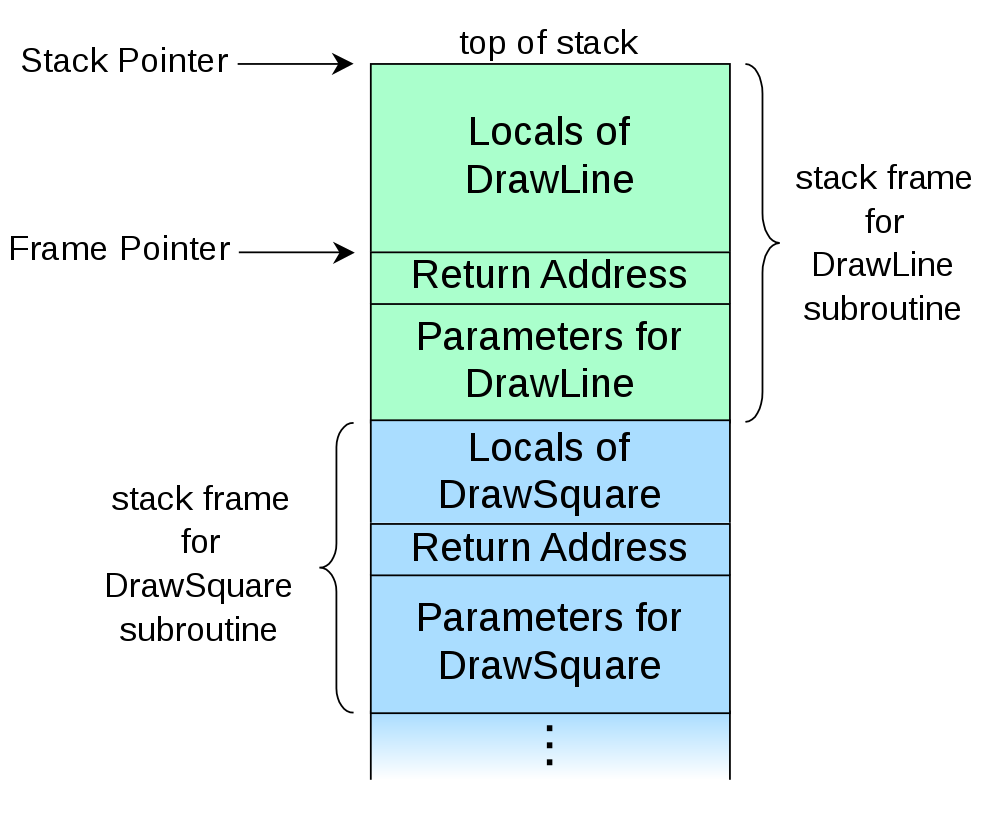
\includegraphics[width=.6\linewidth,keepaspectratio]{art/call-stack-layout.png}
	\caption{Call stack layout for downward-growing stacks\cite{online:stack-img}}
	\label{fig:call-stack-layout}
\end{figure}

The image also shows other important items for proper call stack operations. The \textit{stack pointer} (also in \autoref{fig:x86-regs}) is a CPU register that always points to the top of the stack, at the last accessible address. Another important CPU register is the \textit{frame pointer}, or base pointer (\texttt{rbp}), which points at the base of the currently active stack frame. 

\subsection*{Accessing Thread Execution Stacks}
When using the usual \mintinline{c}|pthread_create()| API function, one simply has to provide a function as a parameter to this newly created thread. Using the default parameters, this call makes the operating system allocate memory for the thread's stack, and then it is scheduled\cite{online:pthread-create}.

It is however possible for users of the POSIX threads library to specify a region of memory to use as the stack space by specifying its attributes with \mintinline{c}|pthread_attr_setstack()|. This simple solution for thread stack execution access by BBPSim was thus chosen. Before starting any flight software thread, \gls{BBPSim} was modified to allocate 2MB of memory for it, which was considered to be sufficient for this application. It should be noted that this block of memory was required to be page-aligned to a virtual memory page. As a result, BBPSim held a reference to every thread's stack. It was then possible to include them in the checkpointing artifact, hence satisfying the third and last necessary condition for a stable restore.

\subsection*{Reconstructing Flight Software Threads}
Once the necessary components were saved as part of the first BBPSim simulation, both the "fresh" and "mature" threads had to be brought back in the same state as they were before. Nevertheless, the past execution stack and register set of a thread weren't enough, by themselves, to be able to restart it. Some meticulous manipulations of that data had first to be done. 

Indeed, the reconstruction of flight software threads had to reconcile two different systems together. From the operating system's point of view, the threads that were spawned in the second simulation run were completely different from those on the first. But from the flight software's perspective, the threads had to be "the same", functionally speaking. In that sense, one couldn't simply copy the old stack onto the new and expect the thread's execution to continue seamlessly. One reason for this is that some important scheduling information was contained at the base of the stack, at higher addresses. 

To solve the problem, this thesis presents a way to reconstruct the old flight software threads by meticulously replacing their stack frames with old frames. 

First of all, it was important to define the concept of \textit{user stack}. The stack of a pthread was divided in four main spaces, like \autoref{fig:stack-spaces} shows. The first two spaces were defined as containing all call frames pertaining to functions in the C and pthread libraries respectively, which use low-level Linux tools to coordinate the creation of the thread. As for the user stack space, it was defined as being the portion that contains all the frames related to \ul{user-defined functions}. In that sense, the \textit{user stack start} was defined as being located at the first 64-bit-aligned address after the pthread stack space. 
\begin{figure}[htbp]
	\centering 
	\includesvg[width=.8\textwidth]{svg/stack-spaces}
	\caption{Division of the execution stack into spaces.}
	\label{fig:stack-spaces}
\end{figure}

Because C code abstracts low-level instructions, finding the beginning of the user stack required the use of assembly. This was done by using \gls{GCC}'s inline assembly tools at the beginning of the first user function (the one provided with \mintinline{c}|pthread_create()|), as \autoref{code:usr-stk-start} shows\cite{online:inline-asm}. Once this address could be accessed, it was possible to deduce the total user stack start offset in any stack $s$ by subtracting the stack top's address:
\[
	\Delta_{usr}=s_{usr}-s_{top}
\]
Once this offset was defined, it was crucial to include it in the checkpointing artifact, since pthreads don't necessarily \textit{always} have the same $\Delta_{usr}$. 
\begin{listing}[htpb]
	\centering
	\begin{minted}{c}
void bbpsimThreadEntry() {
	uint64_t x[4]; //0x20 bytes 
	asm volatile("mov %%rsp, %0  \n\t" //get current stack pointer
                 "addq $0x20, %0 \n\t" 
                 : "=r" (fswthread->m_pi8StartUserStack) //=$s_{usr}$
                 :);
	flightSoftwareTask(); //<- call never returns
}
	\end{minted}
	\caption{Capture of the user stack start.}
	\label{code:usr-stk-start}
\end{listing}

From then, it was possible to reconstruct the thread's execution stack the way it was before by copying only the user and unused portions of the old stack onto the new. This operation was done by the thread itself, using another inline assembly routine located in the restoring function. Since the stack-copying operation had to be done meticulously, it was important not to "pollute" the new stack, and thus this is why assembly was the perfect candidate. The ability to hande the registers manually could provide the required granular control. The complete thread reconstruction routine is included in \autoref{code:stk-copy-asm}. In the code, it is possible to observe many things. First, the \texttt{copyquadword} subroutine (at line \ref{code:copyqword-beg}) is called many times in order to copy the old user stack on the new one, starting from the correct offset. Then the assembly calls \texttt{setcontext()}, which overwrites the current register set with the old one. This call should never return, because it sets the program counter to point back into the flight software code. Because \texttt{setcontext()} itself makes use of the stack\cite{online:setcontext}, it was important to first make the stack pointer point at an appropriate address. In the end, making a live thread replace its own stack frames could qualify as a careful stack corruption exercise, which is pictured in \autoref{fig:stack-reconstruction}.

\begin{figure}[htbp]
	\centering
	\begin{subfigure}{.33\linewidth}
		\centering\small
		\includesvg[height=\linewidth]{svg/stack-reconstruction1}
		\caption{Before copying}
	\end{subfigure}%
	\begin{subfigure}{.33\linewidth}
		\centering\small
		\includesvg[height=\linewidth]{svg/stack-reconstruction2}
		\caption{During copying}
	\end{subfigure}%
	\begin{subfigure}{.33\linewidth}
		\centering\small
		\includesvg[height=\linewidth]{svg/stack-reconstruction3}
		\caption{Copying old frames done}
	\end{subfigure}
	\caption{Stack reconstruction process.}
	\label{fig:stack-reconstruction}
\end{figure}

Keeping in mind that the \gls{BBPSim} library was always loaded at the same address, replacing the entirety of the new user stack by the old one had big benefits:
\begin{itemize}
	\item \textbf{Backtrace information was preserved}. This meant that, when using GDB to debug a simulation, the debugger would correctly find the return addresses in each stack frame (see \autoref{fig:call-stack-layout}) and could thus display the exact call stack that was just restored. The approach "fooled" GDB into thinking this new stack was there all along.
	\item \textbf{Stack variables were preserved}. With the way everything was copied over, even variables allocated on the stack would hold the same value.
\end{itemize}

Using this low-level approach, the restoring of a thread was near instantaneous. The only cost was the stack-copying subroutine, which couldn't really be more optimized than the one in \autoref{code:stk-copy-asm}.

\subsection*{Solution Limitations}
Of course, using such a technique brought its lot of drawbacks. Since the old stack was copied integrally, this meant that pointer variables were put back to hold the same value as before. In flight software, this was mitigated for two reasons: 1. the address of static DAS variables was always the same and 2. dynamic memory allocation wasn't used. However, BBPSim objects were allocated dynamically, and some redefined Deos types had to be modified. This subject is treated in \autoref{cha:bbpsim-impl}. 

This approach was also limited in the fact that \the texttt{-fomit-frame-pointer} GCC option needed to be enabled. Since frame pointers are pushed on the stack when calling a function (in a normal program), this means that the stack usually contains data that points inside \textit{itself}. As thread stacks were dynamically allocated, and thus were never located at the same place in memory, frame pointers were a big problem. Adding the GCC option when compiling every C and \Cpp file completely removes that limitation.



if pointer in stack frame that is copied, need to update it.  Not portable, because assembly. 


When the program is executed, each section gets copied contiguously inside the virtual memory address range allocated for the program by the operating system. 
tried several techniques to save/restore execution stacks:
- strat 3 complicated version of longjmp: how to save execution (asm, disassembly of code, save sp, etc.% https://cs.brown.edu/courses/cs033/docs/guides/x64_cheatsheet.pdf)
Depends on the ABI

